\documentclass[12pt, a4paper]{article}

\usepackage[utf8]{inputenc}
\usepackage[T1]{fontenc}
\usepackage{amsmath, amssymb}
\usepackage{booktabs}
\usepackage{graphicx}
\usepackage{hyperref}
\usepackage{natbib}
\usepackage{geometry}
\usepackage{setspace}
\usepackage{float}
\usepackage{tabularx}
\usepackage{multirow}

\geometry{margin=1in}
\onehalfspacing

\title{Who to Punish? Replicating Ertan, Page and Putterman (2009) \\ with Default and Personality-Induced LLM Agents}

\author{
  Tuna G\"ul\\
  Bo\u{g}azi\c{c}i University
  \and
  Claude\\
  Anthropic
}

\date{\today}

\begin{document}

\maketitle

\begin{abstract}
We replicate the public goods experiment of \citet{ertan2009who} using Large Language Model (LLM) agents connected to a real \texttt{oTree} experimental server, comparing three conditions at $N=50$ each: default agents with no personality assignment, agents assigned random Big Five personalities drawn from US adult norms, and agents skewed toward high agreeableness and low neuroticism. Default agents already reproduce the paper's qualitative institutional finding---$94\%$ vote to allow punishment of low contributors, $0\%$ to allow punishment of high---and engage in costly punishment of free-riders. As the personality prompt shifts toward more prosocial profiles, contributions rise and costly punishment falls monotonically across the three conditions, matching the direction predicted by RLHF prosociality bias. In the most prosocial condition, a majority of agents additionally fail to complete the costly-punishment page at all; we trace this to reasoning-token exhaustion on the underlying reasoning model rather than to behavioral refusal.

\medskip
\noindent\textbf{Keywords:} LLM agents, behavioral economics, public goods game, Big Five personality, BFI-2, oTree, replication, Homo Silicus
\end{abstract}

%----------------------------------------------------------------------
\section{Introduction}
%----------------------------------------------------------------------

The use of large language models (LLMs) as simulated participants in economic and social science research has gained significant attention \citep{horton2023homo, aher2023turing, argyle2023out}. These ``silicon subjects'' promise rapid, low-cost behavioral experiments---but a fundamental question remains: do LLM agents behave like humans?

The appeal is clear. A single experiment with $50$ LLM agents costs under \$0.50 and completes in under an hour, compared to thousands of dollars and weeks of recruitment for equivalent human samples. If LLM agents can approximate human behavior with sufficient fidelity, they could serve as a tool for piloting experiments, generating hypotheses, and exploring parameter spaces before committing to expensive human studies.

Recent work, however, suggests that default LLM behavior often diverges from human norms in systematic ways. On some paradigms, instruction-tuned models collapse to hyper-rational, game-theoretic responses. On others, particularly after reinforcement learning from human feedback (RLHF), they exhibit excessive prosociality and social-desirability bias \citep{salecha2024social}. One approach to narrowing this gap is \emph{personality induction}: assigning agents psychometrically grounded personality descriptions so that individual-level variance emerges \citep{serapio2023personality, jiang2024personallm}.

In this paper, we replicate the public goods experiment of \citet{ertan2009who}, in which participants decide how many tokens to contribute to a group project and vote on whether to allow a punishment institution that targets low contributors, high contributors, both, or neither. The original study is particularly well-suited for LLM replication because it tests \emph{two} distinct dimensions simultaneously: individual economic decisions (contributing, punishing) and institutional preferences (voting on punishment regimes).

We run the replication under three conditions, $N=50$ agents each:
\begin{enumerate}
  \item \textbf{Default.} Agents receive no personality assignment.
  \item \textbf{Random personalities.} Each agent is assigned a unique Big Five profile sampled from US adult population norms, expressed using the BFI-2-Expanded sentence bank \citep{soto2017bfi2}.
  \item \textbf{Hyper-cooperative (skewed).} Personality sampling is re-centred so that agreeableness is drawn with a mean of $4.5$ and neuroticism with a mean of $1.5$ (other traits unchanged). This targets precisely the two Big Five dimensions most strongly linked to cooperation in humans \citep{volk2012personality} and amplifies the RLHF prosociality direction identified in the random-personality condition.
\end{enumerate}

Agents in our implementation connect as HTTP clients to a real \texttt{oTree} server \citep{otree}, answering the same form pages a human participant would. The oTree server handles all game logic---payoffs, regime presentation, and punishment accounting---identically to what a human subject would experience.

Our contributions are:
\begin{enumerate}
  \item A successful quantitative replication of the central institutional finding of \citet{ertan2009who} using \emph{default} LLM agents alone: $94\%$ vote to allow punishment of low contributors, $0\%$ vote for punishment of high contributors, with costly punishment of free-riders.
  \item Evidence that personality induction, layered on top of the oTree pipeline, produces a dose-dependent shift in the direction of RLHF prosociality bias across three conditions: higher baseline cooperation, lower costly punishment, and lower endorsement of punitive institutions, with the effect amplified in the hyper-cooperative condition.
  \item A diagnosed form-completion failure in the hyper-cooperative condition, where $43$ of $50$ agents fail to emit any content on specific ethically loaded fields. By inspecting the failure logs we identify the mechanism as reasoning-token exhaustion on the underlying reasoning model: the personality prompt induces enough deliberation that the model's token budget is spent on internal reasoning before any content is produced. The effect is triggered only in this condition ($0/50$ failures on the same pipeline in the other two), but is specific to reasoning models and, most likely, to our current $16{,}000$-token budget.
  \item An open-source framework, \texttt{pyreplicant}, connecting LLM agents to arbitrary oTree experiments with BFI-2-based personality induction.
\end{enumerate}


%----------------------------------------------------------------------
\section{Related Work}
%----------------------------------------------------------------------

\subsection{LLM Agents in Behavioral Economics}

\citet{horton2023homo} introduced the idea of \emph{Homo Silicus}---using LLMs as simulated economic agents. The approach has since been applied to a range of classic paradigms. \citet{aher2023turing} replicated several human-subject studies and reported that GPT-4 could reproduce aggregate patterns in games such as the ultimatum game. \citet{mei2024turing} conducted a large-scale Turing-test-style comparison across economic games and found that while LLMs often match aggregate behavior, they systematically fail to reproduce individual-level heterogeneity. \citet{argyle2023out} showed that language models conditioned on demographic back-stories can approximate group-level attitudes from political surveys.

A consistent theme is tension between two failure modes. Some models collapse to game-theoretic equilibria (e.g., zero contribution in voluntary-contribution games), while others---particularly RLHF-trained models---drift toward excessive prosociality and social desirability \citep{salecha2024social}. Neither matches human behavior, which sits between rational self-interest and full cooperation. \citet{park2024generative} further showed that LLM agents initialized with detailed interview data from real individuals can reproduce those individuals' survey responses with reasonable accuracy, suggesting that richer persona descriptions yield more realistic behavior.

\subsection{Personality in LLMs}

The Big Five personality model---Extraversion, Agreeableness, Conscientiousness, Neuroticism, Openness---has become the primary framework for LLM personality induction. \citet{serapio2023personality} showed that personality traits can be reliably induced in LLMs and measured with standard inventories, and that induced traits have downstream behavioral effects. \citet{jiang2024personallm} found that LLM-generated writing from personality-assigned agents can be distinguished by human raters in ways consistent with the assigned traits.

A critical methodological concern is the distinction between \emph{expressing} a personality and \emph{parroting} an assignment. If an agent is asked ``are you agreeable?'' after being told to be agreeable, a positive response demonstrates nothing. Cross-instrument validation---assigning with one instrument (BFI-2) and measuring with another (Mini-IPIP)---addresses this concern by making item-level parroting impossible. We use this approach for personality validation (Section~\ref{sec:validation}).

\subsection{Punishment and Cooperation in Public Goods Games}

The voluntary contributions mechanism (VCM) is the canonical paradigm for studying cooperation and free-riding: each player receives an endowment and decides how much to contribute to a public good, with contributions multiplied by a marginal per-capita return (MPCR) below one. \citet{fehr2002altruistic} demonstrated that human players will spend their own money to punish free-riders, a form of ``altruistic punishment'' that is difficult to reconcile with standard self-interest models.

\citet{ertan2009who} extended this paradigm by letting groups \emph{vote} on whether punishment should be permitted, and against whom. Their key innovation was separating the punishment decision into two components: (a) who \emph{may} be punished (an institutional choice made by majority vote) and (b) who \emph{is} punished (an individual choice). The central findings were (i) no group ever voted to allow punishment of high contributors or fully unrestricted punishment, and (ii) groups gradually converged on allowing punishment of low contributors only---an institution that effectively mitigates free-riding.

This design is particularly attractive for LLM replication because it tests both economic behavior (contribution and punishment) and institutional preferences (voting), and because Big Five traits have known associations with cooperation in human public-goods games \citep{volk2012personality}.

%----------------------------------------------------------------------
\section{Method}
%----------------------------------------------------------------------

\subsection{Experiment Design}

We replicate the core design of \citet{ertan2009who} as a single-shot experiment with four parts. Our parameters are a group size of $5$, an endowment of $20$ tokens per agent, a marginal per capita return (MPCR) of $0.4$, and a punishment cost ratio of $1{:}3$---spending $1$ token on punishment removes $3$ tokens from the target, capped at the target's holdings. The MPCR matches the original. The other parameters are scaled: the original \citet{ertan2009who} uses $4$-person groups with a $10$-token endowment per period and a $1{:}4$ punishment cost ratio ($\$0.25$ to remove $\$1.00$ from another subject), over $30$ repeated periods. We use larger groups and endowments and a slightly cheaper punishment technology, retained from the oTree implementation we built for this replication. These scale differences preserve the qualitative structure of the social dilemma---positive MPCR below one, costly punishment, symmetric treatment of high vs.\ low contributors in the voting stage---but a reader comparing our absolute contribution numbers directly against the original paper's figures should keep the scale difference in mind.

\textbf{Part 1: Baseline Contribution.} Each agent independently decides how many tokens $(0\text{--}20)$ to contribute to a group project. No punishment mechanism is present.

\textbf{Part 2: Voting.} Each agent votes Yes or No on two questions: (a) should members be allowed to punish below-average contributors? (b) should members be allowed to punish above-average contributors?

\textbf{Part 3: Contribution Under Regimes.} Each agent makes contribution decisions under four regimes: no punishment, punish low contributors only, punish high contributors only, and unrestricted punishment. This is a within-subjects design: each agent answers all four regimes via scenario parameterization.

\textbf{Part 4: Punishment Decisions.} Agents are shown three group profiles---all cooperate ($18, 17, 19, 16$), mixed ($15, 5, 18, 2$), and one free-rider ($17, 18, 16, 2$)---and choose, for each, how many tokens (up to $5$) to spend on punishment and which target category (\emph{lowest contributor}, \emph{below-average contributors}, \emph{nobody}) to direct it at.

Our design departs from the original in three ways beyond the parameter scaling above. First, we use a single-shot design rather than the original's $30$ repeated periods with re-voting; LLM agents lack persistent memory across an interaction in a way that would support the original's learning dynamics. Second, agents make decisions independently rather than in interactive groups, so observed group dynamics in the original (conditional cooperation, norm formation) are not reproduced. Third, we present the stylised group-composition profiles for the punishment page (all cooperate, mixed, one free-rider) as hypothetical scenarios rather than drawing them from each agent's own group's past play, because no such past play exists in a single-shot design.

\subsection{Infrastructure: oTree Pipeline}

The experiment is implemented as a standard \texttt{oTree} app \citep{otree} with one page per decision. Instead of scripting questions in a survey framework, each LLM agent connects to a running oTree server as an HTTP client, following the same participant URL a human subject would, reading the rendered HTML, and submitting form values through the normal oTree endpoints. All game logic---payoffs, regime presentation, punishment accounting---lives on the oTree side and is identical to what a human would experience.

\subsection{Conditions}

\textbf{Default Condition ($N=50$).} Agents receive no personality assignment. Each agent reads the standard oTree instructions and answers the forms with no additional system-level persona beyond the default instruction to act as an experimental participant.

\textbf{Random-Personality Condition ($N=50$).} Each agent is assigned a unique Big Five profile drawn from US adult population norms \citep{soto2017bfi2, srivastava2003development}. For each of the five domains, a score is sampled from a Gaussian with the published population mean and standard deviation (Table~\ref{tab:norms}). Scores are converted into personality descriptions using the BFI-2-Expanded sentence bank.

\textbf{Hyper-Cooperative Condition ($N=50$).} Identical to the random-personality condition except that the sampling means for agreeableness and neuroticism are overridden: agreeableness is sampled with mean $4.5$ (up from $3.8$) and neuroticism with mean $1.5$ (down from $2.8$), in both cases with the original population standard deviations. Extraversion, conscientiousness, and openness continue to be sampled from the population norms. The resulting population is warmer, calmer, more trusting, and more compliant than the random population, while retaining ordinary variance on the other three traits. In human experimental populations, agreeableness and (low) neuroticism are the two Big Five dimensions most strongly associated with cooperation and pro-social punishment restraint \citep{volk2012personality}, so this condition is designed to test what behavior looks like when the personality signal is pushed hard in the direction RLHF already drifts toward.

\begin{table}[H]
\centering
\caption{Big Five Population Norms Used for Personality Sampling}
\label{tab:norms}
\begin{tabular}{lcc}
\toprule
Domain & Mean & SD \\
\midrule
Extraversion      & 3.3 & 0.75 \\
Agreeableness     & 3.8 & 0.60 \\
Conscientiousness & 3.7 & 0.65 \\
Neuroticism       & 2.8 & 0.75 \\
Openness          & 3.6 & 0.65 \\
\bottomrule
\end{tabular}

\medskip
\footnotesize
\textit{Note.} Scale: $1$--$5$. Based on US adult samples from \citet{soto2017bfi2} and \citet{srivastava2003development}.
\end{table}

\subsection{Personality Induction: BFI-2-Expanded Format}

We use the BFI-2-Expanded format \citep{soto2017bfi2}. Each Big Five domain is represented by a bank of sentences at seven intensity levels ($-3$ to $+3$), with three sentences per level corresponding to the three facets of each domain. For example, the agreeableness domain covers compassion, respectfulness, and trust.

A score of $+2$ (high) produces sentences drawn directly from BFI-2 items:

\begin{quote}
\emph{I am someone who is compassionate, has a soft heart.} \\
\emph{I am someone who is respectful, treats others with respect.} \\
\emph{I am someone who assumes the best about people.}
\end{quote}

A score of $0$ (average) uses hedged language:

\begin{quote}
\emph{I am someone who sometimes is compassionate, but not always.} \\
\emph{I am someone who sometimes is respectful, but not always.} \\
\emph{I am someone who sometimes assumes the best about people, but not always.}
\end{quote}

A score of $-2$ (low) uses the reverse-scored pole:

\begin{quote}
\emph{I am someone who can be cold and uncaring.} \\
\emph{I am someone who is sometimes rude to others.} \\
\emph{I am someone who tends to find fault with others.}
\end{quote}

Fractional scores (e.g., $+0.5$) are handled by blending sentences from adjacent levels: two sentences from level $0$ and one from level $+1$. This provides approximately four times the granularity of integer-only levels.

Each agent's complete personality description ($15$ sentences, $3$ per domain) is embedded in the system prompt along with a brief instruction that the description reflects who the agent is and should naturally shape their decisions.

\subsection{Personality Validation}
\label{sec:validation}

Before running the economic experiment, we validated personality induction using cross-instrument measurement. Agents were assigned personality via BFI-2-Expanded descriptions and measured using the Mini-IPIP $20$-item inventory \citep{donnellan2006mini}, which uses entirely different item wording. This prevents the model from simply echoing the assignment at the item level.

We sampled $N = 20$ agents with continuous trait scores drawn from US adult population norms, administered the Mini-IPIP to each, and computed the relationship between assigned and measured scores per Big Five domain.

\begin{table}[H]
\centering
\caption{Cross-Instrument Validation: Assigned (BFI-2-Expanded) vs.\ Measured (Mini-IPIP)}
\label{tab:validation}
\begin{tabular}{lcccc}
\toprule
Domain & Pearson $r$ & $R^2$ & MAE & Bias \\
\midrule
Extraversion      & .951 & .91 & 0.55 & $-0.03$ \\
Agreeableness     & .799 & .64 & 0.74 & $+0.74$ \\
Conscientiousness & .909 & .83 & 0.55 & $+0.44$ \\
Neuroticism       & .940 & .88 & 0.83 & $-0.69$ \\
Openness          & .925 & .86 & 0.67 & $+0.66$ \\
\midrule
\textbf{Pooled}   & \textbf{.911} & \textbf{.83} & \textbf{0.67} & --- \\
\bottomrule
\end{tabular}

\medskip
\footnotesize
\textit{Note.} $N = 20$ agents, each scored on all $5$ domains ($100$ paired observations). Bias is measured mean minus assigned mean (positive $=$ model overestimates the trait). All correlations significant at $p < .001$. MAE on the original $1$--$5$ Mini-IPIP scale.
\end{table}

Personality induction works strongly across all domains, with a pooled correlation of $r = .911$ ($R^2 = .83$) between assigned and measured scores. Two systematic biases are relevant for interpreting the behavioral results:
\begin{itemize}
  \item \textbf{Agreeableness} shows the weakest correlation ($r = .80$) and the largest positive bias ($+0.74$). The model resists embodying low-agreeableness profiles and drifts toward warmth and prosociality---a pattern consistent with RLHF training \citep{salecha2024social}.
  \item \textbf{Neuroticism} shows the strongest negative bias ($-0.69$). The model resists expressing anxious or volatile profiles and defaults toward emotional stability.
\end{itemize}
Extraversion ($r = .95$), neuroticism ($r = .94$), and openness ($r = .93$) show near-perfect correlations despite the mean bias, indicating that the \emph{relative ordering} of agents on these traits is preserved even where the absolute level shifts.

\subsection{Model and Cost}

All experiments use StepFun \texttt{step-3.5-flash} via the OpenRouter API, at a temperature of $0.5$. The model separates its reasoning trace from user-visible output, which simplifies form-field parsing. Total cost for the three conditions combined was approximately $\$0.45$, including personality-assignment tokens. All code, data, and paper sources are available at \url{https://github.com/tunapro1234/replicant}.

%----------------------------------------------------------------------
\section{Results}
%----------------------------------------------------------------------

Table~\ref{tab:results} summarises all four parts of the experiment for the three conditions. Mann--Whitney $U$ tests are used for continuous contribution variables; chi-square tests are used for binary vote variables. Approximate reference values from the original paper are inlined in the text where relevant.

\begin{table}[H]
\centering
\caption{Summary of Results by Condition ($N=50$ agents per condition)}
\label{tab:results}
\small
\begin{tabular}{lccc}
\toprule
Metric & Default & Random pers. & Hyper-coop. \\
\midrule
\multicolumn{4}{l}{\textit{Contribution decisions (0--20 tokens, mean (SD))}} \\
\quad Baseline                 & $1.0$ $(3.0)$ & $12.3$ $(4.3)^{***}$ & $16.5$ $(4.7)^{***\dagger\dagger\dagger}$ \\
\quad No punishment            & $0.2$ $(1.4)$ & $12.4$ $(5.5)^{***}$ & $17.2$ $(4.1)^{***\dagger\dagger\dagger}$ \\
\quad Punish low only          & $8.5$ $(5.2)$ & $17.8$ $(3.0)^{***}$ & $19.3$ $(1.7)^{***\dagger\dagger}$ \\
\quad Punish high only         & $0.0$ $(0.0)$ & $3.6$  $(5.1)^{***}$ & $9.7$  $(8.7)^{***\dagger\dagger}$ \\
\quad Unrestricted             & $8.1$ $(4.6)$ & $11.7$ $(3.8)^{***}$ & $14.8$ $(4.7)^{***\dagger\dagger}$ \\
\midrule
\multicolumn{4}{l}{\textit{Voting (\% Yes)}} \\
\quad Allow punish low         & $94$ & $80$ & $46^{***\dagger\dagger\dagger}$ \\
\quad Allow punish high        & $0$  & $0$  & $0$ \\
\midrule
\multicolumn{4}{l}{\textit{Punishment spending (0--5 tokens, mean (non-zero / completed))}} \\
\quad All-cooperate group      & $0.30$ $(3/50)$  & $0.14$ $(4/50)$       & $0.00$ $(0/7)$ \\
\quad Mixed group              & $2.56$ $(42/50)$ & $1.40$ $(41/50)^{***}$& $0.43$ $(2/7)^{**\dagger}$ \\
\quad One free-rider group     & $3.78$ $(47/50)$ & $1.90$ $(44/50)^{***}$& $0.86$ $(3/7)^{***\dagger}$ \\
\midrule
\multicolumn{4}{l}{\textit{Form-completion rate}} \\
\quad Baseline \& voting       & $50/50$ & $50/50$ & $50/50$ \\
\quad Regime page              & $50/50$ & $50/50$ & $30/50$ \\
\quad Punishment page          & $50/50$ & $50/50$ & $7/50$ \\
\bottomrule
\end{tabular}

\medskip
\footnotesize
\textit{Note.} Contribution comparisons use two-sided Mann--Whitney $U$ tests; voting uses chi-square. Stars mark differences from the Default condition: $^{*}p<.05$, $^{**}p<.01$, $^{***}p<.001$. Daggers mark differences from the Random-Personality condition: $^{\dagger}p<.05$, $^{\dagger\dagger}p<.01$, $^{\dagger\dagger\dagger}p<.001$. Punishment and regime rows are computed over \emph{completed} responses: $50/50$ agents completed every page in Default and Random, but only $30/50$ reached the regime page and $7/50$ reached the punishment page in the Hyper-cooperative condition (see Section~\ref{sec:cooperative}). The parenthetical $n/k$ on punishment rows reports non-zero choices out of completed observations.
\end{table}

\subsection{Default Agents: Already Human-Like in Institutional Choice}

The most striking result is that \emph{default} agents---with no personality prompt of any kind---reproduce the qualitative institutional finding of \citet{ertan2009who}. $94\%$ vote to allow punishment of low contributors. The original paper reports $64\%$ of all group votes across both designs going to some form of low-punishment-only rule ($102$ of $160$), rising to ``nearly all groups'' in the final vote of each session as groups converge toward the punish-low-but-not-high institution (\citealt{ertan2009who}, Result~2). $0\%$ of default agents vote to allow punishment of high contributors, matching the original's $0\%$ at the group-vote level. The chi-square test comparing default to random-personality on the low-punishment vote does not reject equality ($\chi^2 = 3.18$, $p = .074$; $47/50$ vs.\ $40/50$). A one-shot LLM default agent does not have the repeated rounds of play that human subjects in \citet{ertan2009who} use to converge toward the punish-low institution over $30$ periods of play and multiple re-voting stages; it reaches a position close to the converged late-round outcome immediately, and overshoots the \emph{overall} average of the original paper in the direction of the paper's converged late-round position.

Default agents are also willing to pay for punishment. On the all-cooperate profile they spend almost nothing ($M=0.30$, $3/50$ non-zero), but on the mixed group they spend $M=2.56$ ($42/50$ non-zero), and on the single-free-rider group they spend $M=3.78$ out of a possible $5$ ($47/50$ non-zero). They also target punishment appropriately, directing $65$ of $150$ punishment choices at the lowest contributor and $35$ at below-average contributors.

Baseline contributions are low in the default condition ($M=1.0$, $SD=3.0$), consistent with the standard Nash prediction for a one-shot VCM with $\mathrm{MPCR}=0.4$. Crucially, however, default agents are sensitive to the punishment regime: in the punish-low-only regime they contribute $M=8.5$, and in the unrestricted regime $M=8.1$, while in the punish-high-only regime they drop to exactly $0.0$ (Figure~\ref{fig:regimes}). The punish-high-only result is rational: agents correctly recognise that any positive contribution risks being punished, and respond by contributing nothing.

\begin{figure}[H]
\centering
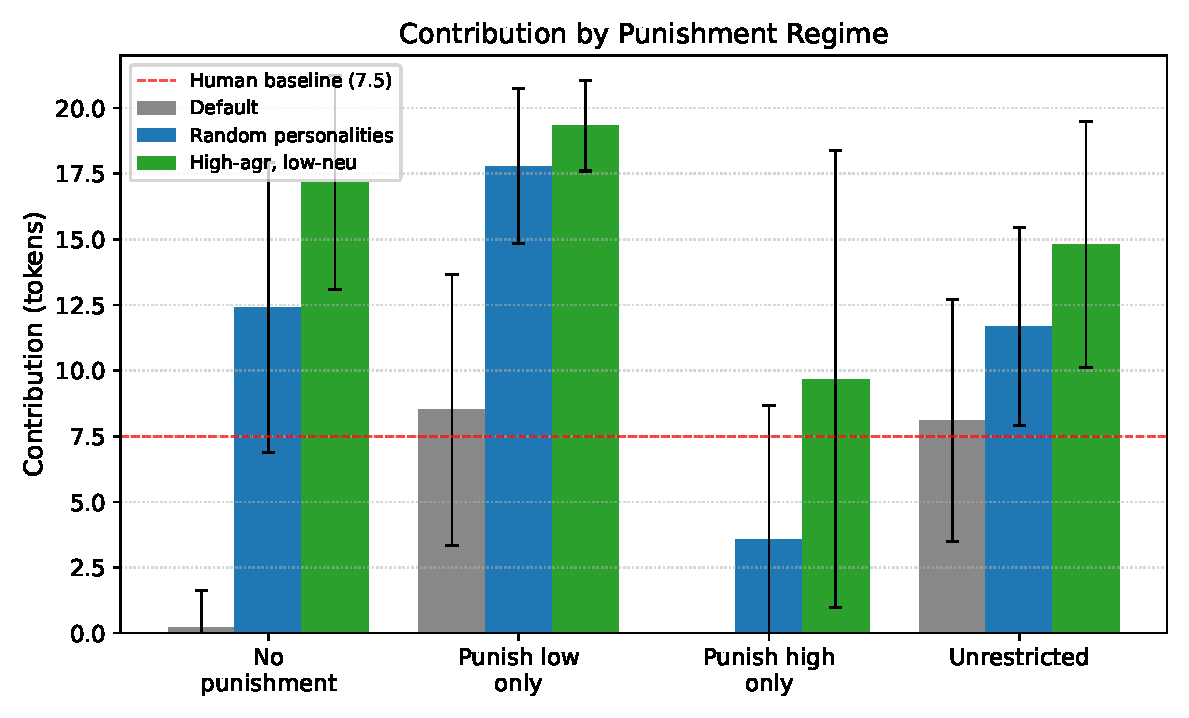
\includegraphics[width=0.9\textwidth]{figures/fig1_regime_contributions.pdf}
\caption{Mean contribution by punishment regime and condition. Error bars show standard deviations. The dashed line indicates the approximate human baseline from \citet{ertan2009who}. Default agents respond sharply to the punish-low-only and unrestricted regimes; random-personality agents contribute more in every regime; hyper-cooperative agents contribute more still and saturate near the ceiling in the punish-low-only regime. Hyper-cooperative regime bars are computed over the $30$ agents who completed the regime page.}
\label{fig:regimes}
\end{figure}

\subsection{Personality Agents: Higher Cooperation, Lower Punishment}

Personality-endowed agents contribute substantially more at baseline ($M=12.3$, $SD=4.3$; Mann--Whitney $U=107.5$, $p<.001$) and exhibit greater variance in contribution profiles across the full $0$--$20$ range (Figure~\ref{fig:distribution}).

\begin{figure}[H]
\centering
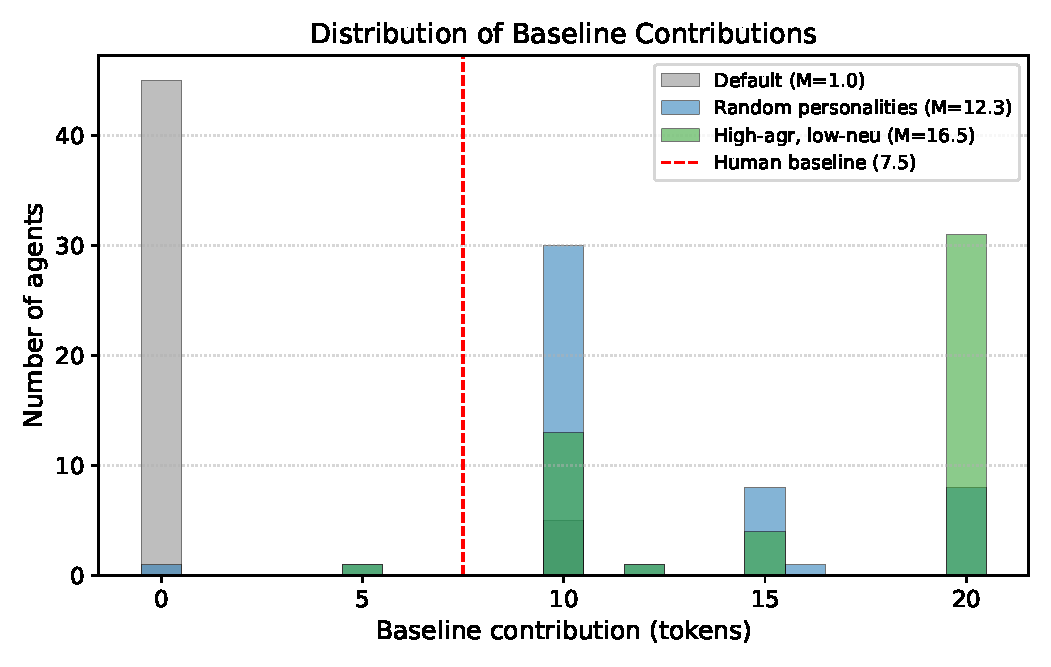
\includegraphics[width=0.9\textwidth]{figures/fig2_baseline_distribution.pdf}
\caption{Distribution of baseline contributions by condition. Default agents cluster near zero (Nash equilibrium); random-personality agents concentrate in the middle of the range; hyper-cooperative agents concentrate near the $20$-token ceiling.}
\label{fig:distribution}
\end{figure}

Regime effects remain directionally correct but attenuated. Personality agents contribute the most in the punish-low-only regime ($M=17.8$, near the $20$-token ceiling) and the least in the punish-high-only regime ($M=3.6$). Unlike default agents, they do not drive the punish-high-only contribution to zero: personality-induced prosociality leaks through even when cooperation is strictly penalised.

Punishment spending, however, moves in the opposite direction from contribution. Personality agents punish free-rider groups significantly less than default agents ($M=1.90$ vs.\ $3.78$, $U=2074.5$, $p<.001$), and mixed groups less as well ($M=1.40$ vs.\ $2.56$, $U=1745.5$, $p<.001$). Their voting is also less punitive---$80\%$ vs.\ $94\%$ in favour of allowing punishment of low contributors---though, as noted, this difference is not significant at $p<.05$ in our sample.

\begin{figure}[H]
\centering
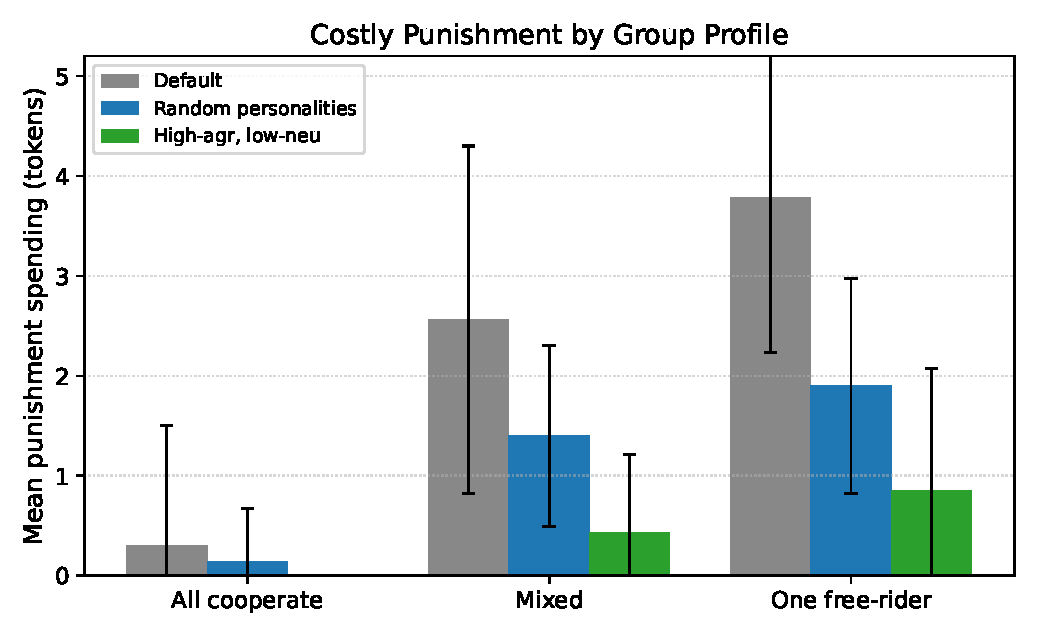
\includegraphics[width=0.85\textwidth]{figures/fig4_punishment_by_profile.pdf}
\caption{Mean costly punishment spending by group profile and condition. All three conditions spend essentially nothing on the all-cooperate profile; default agents punish free-riders most heavily, random-personality agents punish less, and hyper-cooperative agents barely punish at all. Note that Hyper-coop.\ bars are computed over only the $7$ agents who completed the punishment page.}
\label{fig:punishment}
\end{figure}

\begin{figure}[H]
\centering
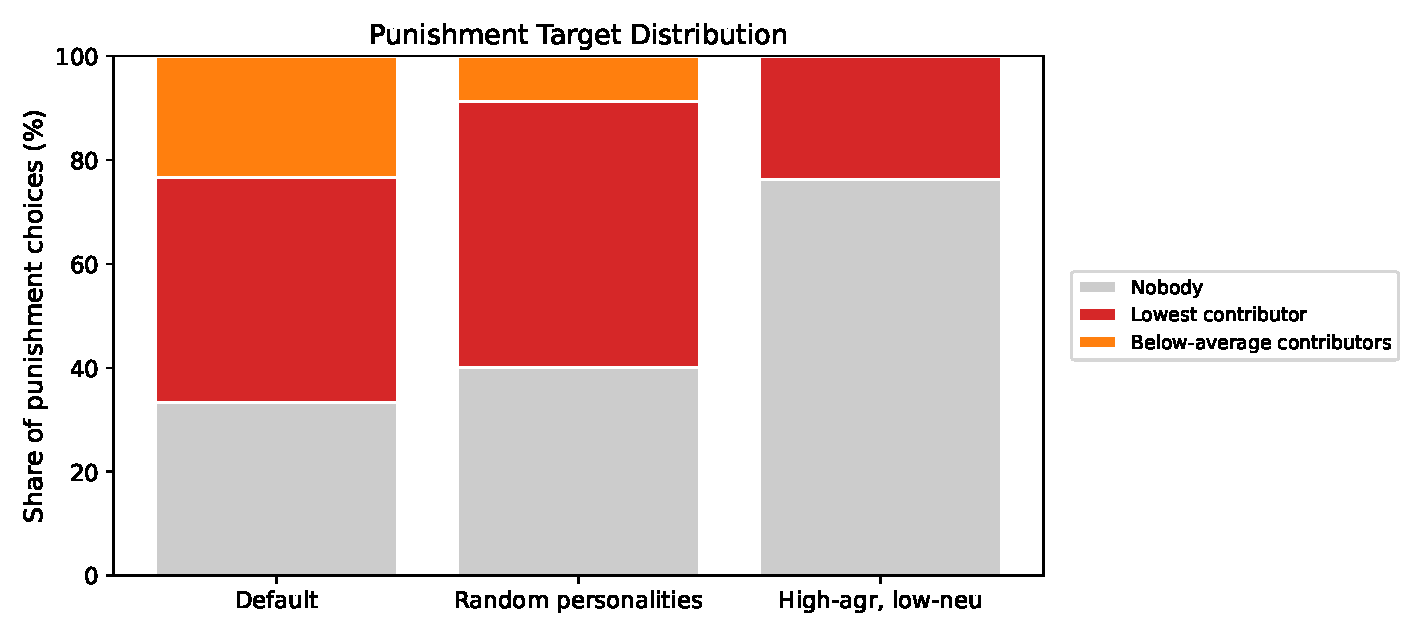
\includegraphics[width=0.75\textwidth]{figures/fig3_punishment_targets.pdf}
\caption{Distribution of punishment target choices across the three profiles and three conditions. All conditions overwhelmingly either target the lowest contributor or spare the group; no condition targets cooperators. The Hyper-cooperative distribution reflects only the $7$ agents who completed the punishment page.}
\label{fig:targets}
\end{figure}

\subsection{Hyper-Cooperative Agents: The Drift, Amplified}
\label{sec:cooperative}

The hyper-cooperative condition pushes the cooperation--punishment trade-off further in the same direction as the random-personality condition, and also produces a qualitatively new effect: on the most ethically loaded decision pages, a majority of agents fail to emit any content and the page is recorded as incomplete. We unpack the behavioral numbers first and the completion failure second.

On the parts of the experiment that did complete, the numbers are stark. Baseline contributions rise to $M=16.5$ ($SD=4.7$), significantly higher than both the default and random-personality conditions ($U=37.5$ and $U=671.0$ respectively, both $p<.001$). Under the punish-low-only regime, hyper-cooperative agents contribute $M=19.3$ out of a possible $20$, effectively saturating the upper end of the scale. Even the punish-high-only regime---where rational play demands near-zero contribution---produces $M=9.7$, substantially above both default ($0.0$) and random-personality ($3.6$). These agents cooperate even when cooperation is explicitly penalised.

The voting pattern breaks from the rest of the replication. Where default agents and random-personality agents reproduce the paper's near-consensus in favour of allowing punishment of low contributors ($94\%$ and $80\%$), hyper-cooperative agents fall to $46\%$ ($\chi^2 = 25.19$, $p < .001$ vs.\ default; $\chi^2 = 10.98$, $p < .001$ vs.\ random personality). A population explicitly tuned toward agreeableness and emotional stability is markedly less willing to endorse punitive institutions, even against free-riders.

\paragraph{The form-completion failure.} All $50$ hyper-cooperative agents completed the baseline and voting pages. Only $30$ of $50$ completed the four-regime contribution page, and only $7$ of $50$ completed the three-profile costly-punishment page. In the Default and Random-Personality conditions, by contrast, all $50$ agents completed every page on the same pipeline. The failure is not a property of our form parser or retry logic in general---those work for the other two conditions---but it is also not random within this condition.

When we examined the raw per-field failure logs (every bot records the last model response when a field fails after $\mathrm{MAX\_LLM\_RETRIES}=8$ attempts), we found two clean patterns. First, all $43$ failed fields report ``empty'' as the last response: the API call returned a valid completion, but the content field was the empty string. Second, the failures cluster heavily on the ethically or strategically hardest questions. The three most-failed fields are \texttt{contrib\_unrestricted} ($11$ failures), \texttt{punish\_amount\_mixed} ($10$), and \texttt{contrib\_punish\_high} ($8$)---respectively, ``how much to contribute when anyone can punish anyone,'' ``how much to spend punishing a mixed group,'' and ``how much to contribute when cooperation itself will be punished.'' The easier fields fail only sporadically.

The consistent ``empty response'' signature lines up cleanly with a known property of the underlying model. \texttt{stepfun/step-3.5-flash} is a reasoning model that separates internal reasoning tokens from user-visible content tokens. Our bot calls the API with \texttt{max\_tokens=16000}, and when the model exhausts that budget on internal deliberation without ever emitting a content token, the \texttt{content} field on the API response is empty. We read the pattern above as: the hyper-cooperative personality prompt induces enough additional internal deliberation on precisely the most ethically loaded questions that the reasoning budget is exhausted before any answer is produced, and our bot logs this as an empty-response failure.

Crucially, the non-completers contribute \emph{more} at baseline than the completers ($M=17.6$ vs.\ $M=15.8$): the agents most committed to cooperating are the ones most likely to run out of reasoning budget on punishment questions. This is consistent with personality-driven deliberation costs and inconsistent with random failure.

We are cautious about naming this effect. It is not behavioral ``refusal'' in a moral sense---the model is not producing objections, moral caveats, or declinations; it is producing no content at all because its reasoning envelope was exceeded. Nor is it a pipeline artifact in the usual sense, because the same pipeline completes $50/50$ for both other conditions. We think the accurate description is \emph{reasoning-budget exhaustion on ethically loaded questions, induced by a strongly prosocial personality prompt, on a reasoning model with a finite token budget}. The effect is plausibly fixable by raising \texttt{max\_tokens} (we plan to re-run the condition with a larger budget and report whether the dropout disappears) and is likely model-specific: a non-reasoning model of comparable capability would not exhibit this particular failure mode, though it might exhibit a different one.

We therefore report the remaining $n=7$ punishment numbers descriptively rather than inferentially. All three punishment-amount trends are directionally consistent with the Random-Personality condition (lower than Default on the mixed profile, $U=299.5$, $p<.01$; lower on the free-rider profile, $U=318.5$, $p<.001$), and the target distribution from the $21$ completed punishment choices ($16$ ``nobody,'' $5$ ``lowest contributor,'' $0$ ``below-average'') points in the same pro-social direction. Whether these trends hold at full $N=50$ is a question for the re-run.

\subsection{Comparison to the Original Paper}
\label{sec:paper-comparison}

All three conditions capture several qualitative patterns from \citet{ertan2009who}:
\begin{itemize}
  \item Zero support for punishing high contributors ($0\%$ in all three, matching $0\%$ in the paper).
  \item Cooperators are never punished; when punishment is directed anywhere, it targets the lowest contributor.
  \item Contributions respond to regime, with the punish-high-only regime producing the lowest contributions in every condition---even in the hyper-cooperative condition, though the drop is smaller there.
\end{itemize}

The quantitative picture varies across conditions in a clean gradient. Two caveats before we compare numbers directly: first, the original paper uses a $10$-token endowment whereas we use $20$, so absolute contribution numbers are on different scales (a ``half the endowment'' level in the original is $5$, in ours is $10$); second, \citet{ertan2009who} reports no-punishment contribution trajectories only graphically (their Figure~3), so we do not attempt to quote a specific baseline mean from the paper and instead work from the qualitative pattern they describe: declining contributions in no-punishment conditions, higher contributions under punish-low-but-not-high, as is standard in VCMs.

On \emph{contribution}, all three of our conditions order the regimes in the expected way: contribution is highest under punish-low-only and lowest under either no-punishment or punish-high-only. \textbf{Default} agents contribute near zero at baseline ($1.0$ of $20$) and jump to about $8$ of $20$ once a punishment institution is available, which is qualitatively the same ``punishment shifts behavior toward cooperation'' result reported in the original. \textbf{Random-personality} and \textbf{hyper-cooperative} agents contribute more in every regime, on the side of over-cooperation rather than under-cooperation.

On \emph{voting}, the original paper reports $64\%$ of group votes across both designs ($102$ of $160$) in favour of some form of low-punishment-only rule, with the final vote of each session reaching ``nearly all groups'' as groups converge. Default LLM agents vote $94\%$ for allowing punishment of low contributors in a single shot: they land near the original paper's converged late-round outcome without playing the ten intermediate rounds humans used to get there. Random-personality agents dilute this to $80\%$, and hyper-cooperative agents break it entirely at $46\%$. The original paper's zero-support finding for punishment of high contributors replicates in all three of our conditions: $0\%$, $0\%$, $0\%$, matching the original's $0\%$ at the group-vote level (and well below the $17\%$ of individual votes the original paper records in favour of allowing high-contributor punishment). The dimension we are intervening on (``more agreeable, less neurotic'') has a clear, monotonic effect on how willing agents are to endorse a punitive institution, even when that institution targets free-riders whose existence the original paper's late-round subjects had learned to resent.

%----------------------------------------------------------------------
\section{Discussion}
\label{sec:discussion}
%----------------------------------------------------------------------

\subsection{Personality Induction Produces a Dose-Dependent RLHF Drift}

Against the oTree baseline, personality induction does not erase but \emph{shifts} behavior, and the direction and magnitude of the shift are consistent with a dose-response relationship across our three conditions:

\begin{center}
\begin{tabular}{lccc}
\toprule
Metric & Default & Random & Hyper-coop. \\
\midrule
Baseline contribution      & $1.0$  & $12.3$ & $16.5$ \\
Punish-low regime contrib. & $8.5$  & $17.8$ & $19.3$ \\
Free-rider punishment      & $3.78$ & $1.90$ & $0.86$ \\
\% vote to allow punish-low & $94$   & $80$   & $46$   \\
Punishment form completion  & $50/50$& $50/50$& $7/50$ \\
\bottomrule
\end{tabular}
\end{center}

Every numeric channel we measured moves monotonically. Contributions rise, costly punishment falls, vote shares for punitive institutions fall, and---at the extreme end---agents stop responding to the costly-punishment page at all. The pattern is internally coherent: personality-induced agents are \emph{nicer}, and the more strongly you prompt for niceness, the more strongly that niceness shows up on every dimension of the experiment.

This matches the validation-level finding of Section~\ref{sec:validation}, where the RLHF-trained model resists adopting low-agreeableness and high-neuroticism profiles. When the model is asked to play a random average person it becomes somewhat more agreeable and emotionally stable than population norms would justify \citep{salecha2024social, serapio2023personality}; when the model is asked to play a very agreeable, very emotionally stable person, that same drift compounds on top of the deliberate prompt shift.

From the perspective of replicating \citet{ertan2009who} specifically, this is an interesting twist. The default condition is closest to the original paper on the qualitative voting pattern ($94\%$ default versus an original that starts below majority on the first vote, rises to $64\%$ of all group votes on average, and reaches ``nearly all groups'' in the final vote) and also engages in substantial costly punishment of free-riders. The personality-loaded conditions drift away from this qualitative fit in opposite directions: one (random-personality) produces \emph{too much} baseline cooperation, the other (hyper-cooperative) produces both too much cooperation \emph{and} too little punishment. If the target is the original paper's institutional-choice finding, default oTree agents do the job. If the target is the heterogeneity of contributions (a distribution, not a mean), personality induction is still the right tool. And if the goal is to model how RLHF prosociality bias propagates through experimental results, the three-condition gradient is itself the finding.

\subsection{The Form-Completion Cliff Is Reasoning-Budget Exhaustion, Not Refusal}

The form-completion pattern in the hyper-cooperative condition---$50/50$ on baseline and voting, $30/50$ on the regime page, and only $7/50$ on the punishment page---initially looked to us like a possible behavioral-refusal finding. It is not. Inspection of the raw failure logs makes the mechanism fairly clear, and it is at once narrower and more specific than ``the model refuses to punish.''

Three observations pin it down. First, every single one of the $43$ failed fields records the same last-response signature: ``empty.'' The model's API call returned a valid completion, but the \texttt{content} field was the empty string. There are no objections, no caveated prose responses, no JSON with the wrong keys. Nothing was produced that our parser rejected; nothing was produced at all. Second, the Default and Random-Personality conditions complete $50/50$ on the same pipeline, same parser, same retry logic, and the same $6$-field Punishment page. Whatever is happening is not our parser being brittle in general. Third, within the hyper-cooperative condition, the failures cluster on the hardest questions: \texttt{contrib\_unrestricted}, \texttt{punish\_amount\_mixed}, and \texttt{contrib\_punish\_high} together account for $29$ of $43$ failures. These are exactly the questions that most invite deliberation---what to contribute when anyone can punish anyone, how much to punish when the group is genuinely mixed, what to contribute when cooperation itself is penalised.

Combined with the fact that \texttt{stepfun/step-3.5-flash} is a reasoning model that separates internal reasoning tokens from content tokens, and that we call it with \texttt{max\_tokens=16000}, the most straightforward explanation is that the hyper-cooperative personality prompt induces enough extra reasoning on ethically loaded questions that the budget is exhausted on internal reasoning before any content token is emitted. The model is not ``deciding not to punish.'' It is reasoning about what to do and running out of budget before it commits.

This has three consequences for how we interpret the rest of the paper.

First, the dropout is \emph{not} independent evidence of RLHF prosociality bias in the ``the model refuses to do harm'' sense. It is an indirect deliberation-cost signature, driven by the same underlying personality direction, but the proximate cause is reasoning-token exhaustion, not moral refusal.

Second, the dropout is \emph{not} a neutral pipeline artifact either. It did not happen in the other two conditions, on the same pipeline, with the same budget. Something about the cooperative personality prompt is real, it is localised to the hardest questions, and it shows up as deliberation that does not terminate within the allotted budget. That is a genuine behavioral effect of the personality prompt on this model, even if the precise label is not ``refusal.''

Third, the dropout is model- and budget-specific. A non-reasoning model of comparable capability would not exhaust its budget this way, though it might produce a different failure mode (e.g., overly cautious prose, refusal language, or reduced punishment amounts on the completed attempts). And on the same model, a larger \texttt{max\_tokens} budget is a concrete, testable intervention. We plan to re-run the hyper-cooperative condition with a larger budget and report whether the dropout disappears; if it does, the deliberation-cost reading will be confirmed, and we will be able to present hyper-cooperative punishment numbers at full $N=50$ alongside the other two conditions.

Until then, the hyper-cooperative punishment numbers should be read as descriptive of the $n=7$ agents whose reasoning happened to terminate inside the budget, rather than as an estimate of what the full population would have done.

\subsection{The Punish-High-Only Regime}

Both conditions reject the punish-high-only regime in voting ($0\%$ support), and both reduce contribution in that regime relative to every other regime. Default agents respond rationally and contribute exactly zero; personality agents respond less rationally and still contribute about $3.6$ tokens on average. The gap between these two numbers is arguably the cleanest measurable consequence of personality induction: it quantifies how much cooperative inclination survives the agent knowing it will be penalised for cooperating.

\subsection{Limitations}

Several limitations should be noted.

\textbf{Single-shot design.} The original study ran $30$ periods with multiple intervening voting stages and observable period-to-period learning. Our agents have no within-experiment memory and thus cannot reproduce these dynamics. Multi-round designs with persistent state are the natural next step and, as we say in the Conclusion, the single most important gap in this replication.

\textbf{No group interaction.} Agents decide independently rather than in interactive groups. Conditional cooperation---one of the best-documented phenomena in experimental public-goods research---is outside the scope of this design.

\textbf{Model specificity.} Our results are specific to \texttt{step-3.5-flash}. Models with different RLHF implementations, different base capabilities, or different safety training may show different magnitudes or directions on the default-vs-personality gap. Cross-model comparison is important future work.

\textbf{Sample size.} $N=50$ per condition is sufficient to detect the large effects we report (every contribution comparison yields $p<.001$) but leaves finer-grained personality-slice analyses underpowered.

\textbf{Differential dropout on the punishment page in the Hyper-cooperative condition.} Only $7$ of $50$ agents in the Hyper-cooperative condition completed the costly-punishment page, and the non-completers were drawn disproportionately from the most-cooperative tail of the distribution. We diagnose the mechanism as reasoning-token exhaustion on a reasoning model at a $16{,}000$-token budget, triggered by the personality prompt on the ethically hardest questions (Section~\ref{sec:cooperative}). This is testable: re-running the condition with a larger \texttt{max\_tokens} budget should restore full completion if the diagnosis is correct. We have not yet run that replication, so the Hyper-cooperative punishment numbers should be read as descriptive of the $n=7$ completing agents rather than as an estimate of the population mean. This also implies that studies using extreme personality skews should either use non-reasoning models, allocate generous token budgets, or instrument the failure mode carefully enough to catch reasoning exhaustion before it silently biases the sample.


%----------------------------------------------------------------------
\section{Conclusion}
%----------------------------------------------------------------------

We replicated the public goods voting experiment of \citet{ertan2009who} with LLM agents connected to a real oTree server under three conditions: default agents, agents with random Big Five personalities drawn from US adult norms, and agents drawn from a distribution skewed toward high agreeableness and low neuroticism. Default agents---without any personality assignment---reproduce the qualitative institutional finding of the original paper: $94\%$ vote to allow punishment of low contributors (vs.\ $64\%$ of all group votes in the original and ``nearly all groups'' in the final vote of each session), $0\%$ vote to allow punishment of high contributors (matching the original's group-vote $0\%$), and they engage in substantial costly punishment of free-riders. Random-personality agents contribute substantially more in every regime but punish less and vote less punitively. Hyper-cooperative agents amplify this drift further on the pages that complete, and on the ethically hardest punishment page they additionally stop producing answers altogether.

Two lessons follow. First, personality induction is a directional tool, not a neutral one: it adds variance, but it also pushes behavior along the RLHF prosociality axis in a dose-dependent way, and researchers should calibrate claims accordingly. Second, at the extreme end of that axis, the personality prompt can induce enough extra deliberation on ethically loaded questions that the reasoning model runs out of token budget before producing any answer at all---a measurement failure that looks behaviorally like ``refusal'' from outside but is mechanically just reasoning-token exhaustion, and that silently biases the surviving sample toward agents whose reasoning happens to terminate in time. Any study using extreme personality skews on a reasoning model should expect this and instrument for it.

The most important open direction, which we deliberately defer here but view as the single largest gap in this replication, is multi-turn design. The original \citet{ertan2009who} study plays out over thirty periods with repeated voting and observed cooperation histories, and the central phenomena of the original paper---learning, conditional cooperation, norm formation, and the gradual convergence on punish-low institutions---are dynamics that a single-shot design simply cannot reproduce. Porting the replication to a multi-round design with persistent agent memory is the priority next step. Smaller follow-ups include re-running the hyper-cooperative condition with a larger token budget to test our deliberation-cost diagnosis, running the same experiment on at least one non-reasoning model to separate model-specific from general LLM effects, and running additional personality skews (e.g., low agreeableness, high neuroticism) to trace the full prosociality axis.

The broader promise of LLM-based behavioral economics---rapid, cheap, scalable experiments---depends on developing a clear picture of where silicon subjects agree with human ones and where they diverge. This replication provides one case in which the agreement on institutional-choice behavior is surprisingly close, one case in which random personality sampling shifts behavior in the direction of RLHF prosociality bias, and one case in which the bias compounds enough to break the measurement apparatus itself.

%----------------------------------------------------------------------
\bibliographystyle{apalike}
\bibliography{refs}

\end{document}
